\documentclass[spanish,notitlepage,letterpaper, 10pt]{article} % para articulo en castellano
\usepackage{cite}
\usepackage[utf8]{inputenc} % Acepta caracteres en castellano
\usepackage[spanish]{babel} % silabea palabras castellanas
\usepackage{amsmath}
\usepackage{here}

\usepackage{amsfonts}
\usepackage{amssymb}
\usepackage{hyperref} % navega por el doc
\usepackage{graphicx}
\usepackage{geometry}      % See geometry.pdf to learn the layout options.
\geometry{letterpaper}                   % ... or a4paper or a5paper or ... 
%\geometry{landscape}                % Activate for for rotated page geometry
%\usepackage[parfill]{parskip}    % Activate to begin paragraphs with an empty line rather than an indent
\usepackage{epstopdf}
\usepackage{fancyhdr} % encabezados y pies de pg

\usepackage{listings}
\usepackage{color}

\definecolor{dkgreen}{rgb}{0,0.6,0}
\definecolor{gray}{rgb}{0.5,0.5,0.5}
\definecolor{mauve}{rgb}{0.58,0,0.82}

\lstset{frame=shadowbox,
  language=matlab,
  aboveskip=3mm,
  belowskip=3mm,
  showstringspaces=false,
  columns=flexible,
  basicstyle={\small\ttfamily},
  numbers=left,
  numberstyle=\tiny\color{gray},
  keywordstyle=\color{blue},
  commentstyle=\color{dkgreen},
  stringstyle=\color{mauve},
  breaklines=true,
  breakatwhitespace=true
  tabsize=3
  rulesepcolor=\color{blue}
}

\newcommand{\university}{\normalsize Universidad Industrial de Santander}
\newcommand{\faculty}{\normalsize  Escuela de Ingenier\'ia de Sistemas e Inform\'atica}
\newcommand{\codigo}{\normalsize  2182066}
\newcommand{\grupo}{\normalsize  B2}
\pagestyle{fancy} 
\chead{\bfseries Lab. } 
\lhead{} % si se omite coloca el nombre de la seccion
\rhead{\today} 
\lfoot{\it  An\'alisis N\'umerico } 
\cfoot{\university} 
\rfoot{\thepage} 

\voffset = -0.25in 
\textwidth = 7.5in
\textheight = 9in
\oddsidemargin = -0.5in
\headheight = 20pt 
\headwidth = 7.5in
\renewcommand{\headrulewidth}{0.5pt}
\renewcommand{\footrulewidth}{0,5pt}
\DeclareGraphicsRule{.tif}{png}{.png}{`convert #1 `dirname #1`/`basename #1 .tif`.png}


\begin{document}

\title{	\vspace{-12mm}
\includegraphics[width=0.2\linewidth]{Logos/UIS.pdf}\\Informe Laboratorio: Análisis Numérico\\  \centering Práctica No. 1}
\author{
\textbf{Daniel Delgado} \\ \textbf{Código:} \codigo\\
\textbf{Grupo:} \grupo\\
\textit{\faculty}\\
\textit{\university}}
\date{\today}
\maketitle

\section{Introducción}
Los puntos fijos, o \textit{fixed points}, están definidos como puntos dentro de una función donde este, al ser evaluado en la misma función, dará como resultado a sí mismo. Matemáticamente hablando, nos referimos a un punto $x$ para el cual $g(x)=x$. 

Esta propiedad de estos números considerados puntos fijos son utilizados el múltiples áreas de las ciencias básicas, como lo viene siendo la biología, química y física; las ciencias aplicadas, como las ciencias de computación y algunas ingenierías; e incluso algunas ciencias humanas, como es el caso de la economía.

La comprensión de los conceptos de los puntos fijos, y el método iterativo empleado de manera computacional para el cálculo de estos, son los principales temas a tratar en el presente informe de laboratorio, así como la resolución de los problemas propuestos a manera de pregunta orientadora durante el desarrollo de la parte práctica del mismo.  

\section{Desarrollo}
\begin{enumerate}
  \item \textbf{Preguntas propuestas}
    De manera inicial, la guía de laboratorio propone las siguientes preguntas con el fin de llevar más allá la comprensión de los conceptos trabajados durante el desarrollo práctico del laboratorio.
    \begin{enumerate}
      \item ¿Qué es un punto fijo?
        
        Bajo el contexto matemático, el concepto de punto fijo está definido como un punto $k \in [a,b]$ para una función continua $g(x)$ en el cual $g(k) = k$. 
      
      \item ¿Cómo se calcula un punto fijo?
      
        Un punto fijo puede calcularse de varias maneras, sin embargo, en este caso se está empleando el método iterativo para realizar el cálculo de un punto fijo. Este se basa en calcular el valor de un punto fijo a partir de un punto inicial, tomar el resultado obtenido tras la primera computación del valor y usarlo en el siguiente cálculo. Esto se repite hasta hallar el valor del punto fijo.

      \item ¿Qué aplicaciones tiene el método de punto fijo?
      
      El método de punto fijo, de manera general tiene múltiples aplicaciones en campos que van desde la economía, donde es aplicado en El equilibrio de Nash \cite{nash}; hasta en las ciencias de la computación, donde tiene aplicaciones dentro de la teoría de tipos en cuanto a funciones recursivas se refiere. \cite{combinator}     

      \item ¿Qué condición debe satisfacerse para garantizar que una función tiene un punto fijo?
      
      La condición que deber satisfacerse para determinar si una función tiene un punto fijo es que, para una función $g(x)$ continua sobre un intervalo $[a,b]$, el rango de esta función es $[a,b]$, la función tendrá un punto fijo sobre $[a,b]$

      \item ¿Qué condición debe satisfacerse para garantizar que un punto fijo es único?
      
      La manera de garantizar que exista un único punto fijo es que el valor absoluto de la derivada de $g(x)$ para un punto fijo $k \in [a,b]$ sea menor que 1, es decir, $|g'(x)| < 1$.

    \end{enumerate} 
  \item \textbf{Aplicando de manera manual}
  
  Con el propósito de ver en acción el método iterativo, se realizarán 5 iteraciones a mano para la función $f(x)=1-\frac{x^2}{4}$.

  Tomando $P_0 = 1$ 
  \begin{center}
    
    $P_0 = 1$ \\
    $g(P_0) = 1-\frac{1^2}{4} = 1-\frac{1}{4} = \frac{3}{4} = 0.75 = P_1$ \\
    $g(P_1) = 1-\frac{0.75^2}{4} = 1 - \frac{9}{64} = \frac{55}{64} = 0.859375 = P_2 $ \\
    $g(P_2) = 1-\frac{0.859375^2}{4} = 0.815368652343750 = P_3$ \\
    $g(P_3) = 1-\frac{0.815368652343750^2}{4} = 0.833793490193784 = P_4$ \\
    $g(P_4) = 1-\frac{0.833793490193784^2}{4} = 0.826197103927617 = P_5$

  \end{center}

  Como puede observarse, de esta manera estamos iterando sobre los diferentes resultados obtenidos por lo que, eventualmente, con un suficiente número de iteraciones, para este caso específico, será posible determinar el punto fijo entre $[0,1]$.

  \item \textbf{Implementación de algoritmia}

  Una de las partes más importantes respecto al desarrollo del trabajo de laboratorio en cuanto a su componente práctico se refiere a la implementación de algoritmia con el fin de cumplir con un objeto o dar solución a un problema propuesto.

  \begin{enumerate}
    \item Determinación del punto fijo de manera iterativa
    
    De manera inicial se buscó desarrollar un algoritmo el cual realizara el proceso iterativo en la búsqueda de un punto fijo dentro de un rango determinado y un número de iteraciones definidas. Esto fue realizado con la función \texttt{fixedPoint(aFunction, lowerLimit, upperLimit, initalPoint, iterations)}. 

    \begin{lstlisting}
function output = fixedPoint(aFunction, lowerLimit, upperLimit, initalPoint, iterations)
  %Check inputs for errors%
  if ((lowerLimit < upperLimit) && (0 < iterations) && (lowerLimit <= initalPoint <= upperLimit) && isa(aFunction, 'function_handle'))
    output = initalPoint;
    for index = 1:iterations
      older = output;
      output = aFunction(output);
      if (lowerLimit <= output <= upperLimit) 
        if older == output
          disp('fixed point was found:')
          disp(output)
          return;
        end
      else
        warning('given function breaks out of stablished range')
        return;
      end
    end
    if older-output == 0
      %just to avoid fun things
    elseif (abs(older - output) < 0.00001)
      disp(['A possible fixed point was found close to ', output, '. More iterations might confirm if it is a fixed point.'])
      output = NaN;
    else
      disp('A fixed point was not found. Increasing the number of iterations could help locating one but it is not completely certain.')
      disp('It is also possible than the given function fixed points can not be calculated using the iterative method.')
      output = NaN;
    end
  else
    warning('Error! Given arguments for function fixedPoint are not valid!')
    output = NaN;
  end
end
    \end{lstlisting}

    En cuanto al como funciona el algoritmo, de manera inicial, la función realiza algunas verificaciones de los parámetros dados con el fin de evitar errores en cuanto a la ejecución se refiere. Asumiendo que los parámetros dados son validos, se procede a iniciar el ciclo iterativo con el cual se calculará el valor del punto fijo.
    
    Dentro del ciclo iterativo se tomará \texttt{older} como el valor de $P_{n-1}$ como se puede ver en la línea 6 donde, antes de realizar el cálculo del nuevo valor para output $(P_n)$ en la línea 7, esta se iguala con output. Tras esto, se harán algunas comprobaciones respecto al valor de \texttt{output} en cuanto a si este sigue dentro del dominio establecido, al igual de revisar si se ha encontrado un punto fijo. Finalmente, se volverá al inicio del ciclo iterativo repitiendo el mismo proceso hasta que se encuentre un punto fijo o se realicen todas las iteraciones.

    \item Comprobación visual de un punto fijo
    
    En la segunda parte, era necesario el graficar una función dentro de un dominio dado con el fin de verificar de manera gráfica la existencia de puntos fijos. Esto se realizó con la función
    \texttt{visualVerification(aFunction, lowerLimit, upperLimit)}.

    \begin{lstlisting}
function output = visualVerification(aFunction, lowerLimit, upperLimit)
  %Check inputs for errors%
  if (isa(aFunction, 'function_handle') && (lowerLimit < upperLimit))
    domain = [lowerLimit, upperLimit];
    range = aFunction;
    straightLineFunction = @(x)x;
    fplot(range, domain)
    hold on
    fplot(straightLineFunction, domain)
    set(get(gca, 'XLabel'), 'String', 'X');
    set(get(gca, 'YLabel'), 'String', 'Y');
    set(get(gca, 'Title'), 'String', 'Visual Verification');
  else 
    warning('Error! Given arguments for function visualVerification are not valid!')
    output = NaN;
  end
end
    \end{lstlisting}

    Esta función, en esencia, realiza dos simples tareas: la primera es la verificación de los parámetros dados, como puede verse en la línea 3; y la graficación de la función pasada como parámetro y una recta definida por la función $p(x) = x$ como se ve en de la línea 9 a la 11. El resultado es la gráfica presente en la Fig. \ref{visual}.

    \begin{figure}[H]
      \centering
      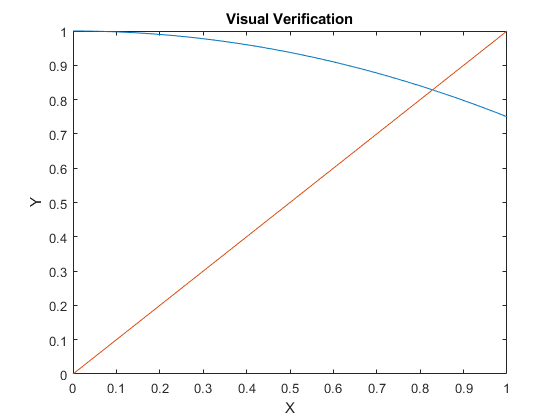
\includegraphics[width=8cm]{Images/visual.png}
      \caption{Gráfica generada por la función \texttt{visualVerification}}
      \label{visual}
    \end{figure}

    \item implementación para un caso específico
    
    Finalmente, se realiza la aplicación de las funciones planteadas para la función $g(x) = 1+\frac{2}{x}$ en el dominio $[1,5]$. Con el fin de unificar el proceso dado, se realizó una tercera función \texttt{fixedPointV2(aFunction, lowerLimit, upperLimit, initalPoint, iterations)} la cual se aplica \texttt{fixedPoint} de manera normal pero se agrega la función \texttt{visualVerification} en el caso de que se encuentre un punto fijo como se evidencia de la línea 9 a la 14.

    \begin{lstlisting}
function output = fixedPointV2(aFunction, lowerLimit, upperLimit, initalPoint, iterations)
  output = fixedPoint(aFunction, lowerLimit, upperLimit, initalPoint, iterations);
  if isnan(output)
    return;
  else
    visualVerification(aFunction, lowerLimit, upperLimit);
  end
 end
    \end{lstlisting}

    Al ingresar en la consola de matlab: \texttt{fixedPointV2(@(x)1+(2/x),1,5,4,100)}, podemos ver como retorna \texttt{ans = 2} y la figura \ref{FiguraCool}.

    \begin{figure}[H]
      \centering
      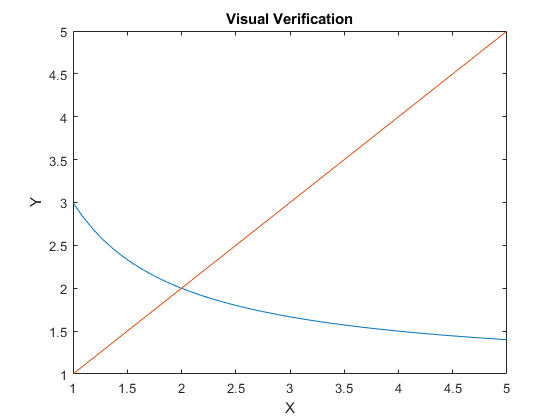
\includegraphics[width=8cm]{Images/taco.png}
      \caption{Gráfica generada por la función \texttt{fixedPointV2}}
      \label{FiguraCool}
    \end{figure}

  \end{enumerate}

  \item \textbf{Interpretación de un problema}
  
  La siguiente parte se basa en el planteamiento de un problema específico. En este, se nos pide, empleando las funciones anteriormente planteadas, para calcular cuando se generaba una congestión en el sistema. Esta la velocidad con la que se asignaba la información estaba definida por la función $u_{4.8}(x)=(4.8)log(x)$. 
  
  Entonces, con el fin de resolver el problema, se empleó la función \texttt{fixedPoint(@(x) 4.8*log(x),5,15,10,100)}. El resultado obtenido tras computar la función fue \texttt{ans = 11.878842680112935} y dió la gráfica presente en la Fig. \ref{interp}. Es decir que la congestión del sistema se dará cuando $x = 11.878842680112935$. 

  \begin{figure}[H]
    \centering
    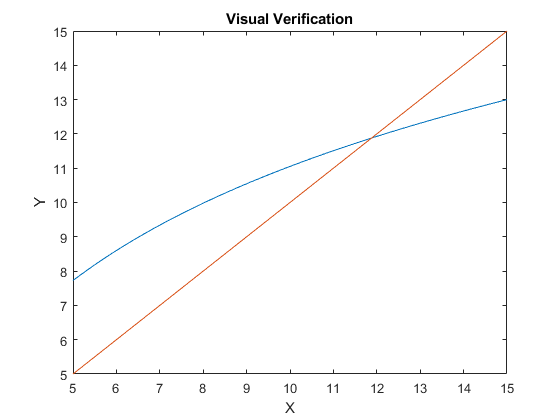
\includegraphics[width=8cm]{Images/interpretando.png}
    \caption{Gráfica generada por la función \texttt{fixedPoint}}
    \label{interp}
  \end{figure}
  
  \item \textbf{Propuesta de aplicación}
  
  \begin{enumerate}
    \item \textbf{Un problema hipotético}
    
    Las temperaturas internas de un nuevo prototípo de procesador impactan fuertemente el rendimiento de este. El rendimiento relativo de este está definido por la función $c(x) = 1-\frac{1}{40}x-\frac{1}{8}\left(x\right)^{2}$. Tras muchos estudios, se encontró que la mejor manera, tanto por factibilidad de construcción y limitaciones de la tecnología empleada, era cuando la temperatura en unidades arbitrarias y el rendimiento relativo del procesador eran básicamente iguales. ¿Qué temperatura relativa es la ideal teniendo en cuenta que el mínimo de esta temperatura 0 hasta 2.5 unidades arbitrarias? 

    \item \textbf{Resolución del problema}
    
    Por el como está planteado el problema, es evidente que la temperatura óptima para el procesador está presente en un punto fijo. En este orden de ideas, podemos aplicar la función \texttt{fixedPointV2} con el fin de obtener tanto el resultado del punto fijo necesario al igual que una gráfica para realizar la comprobación visual del mismo. 

    En este orden de ideas, se pasaron los siguientes parámetros a la función.

    \begin{lstlisting}
f = @(x)1-((1/40)*x)-((1/8)*x^2);
l = 0;
u = 2.5;
t = 1;
r = 5000;
fixedPointV2(f,l,u,t,r)
    \end{lstlisting}

    Tras aplicar la función, el resultante sería \texttt{ans = 0.880963762164909} y la gráfica de la Fig. \ref{final}.
  

    \begin{figure}[H]
      \centering
      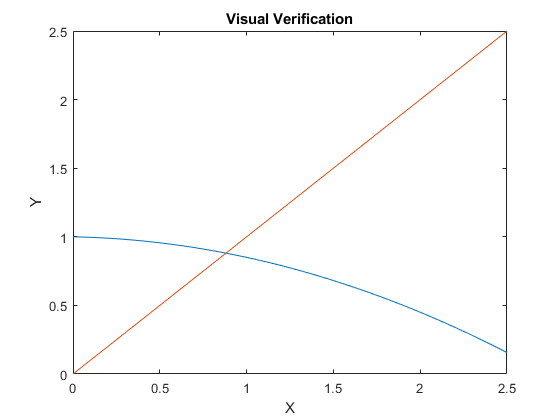
\includegraphics[width=8cm]{Images/fin.png}
      \caption{Gráfica generada por \texttt{FixedPointV2}}
      \label{final}
    \end{figure}
  
  \end{enumerate}

\end{enumerate}

\section{Anexos}

Ver fixedPoint.m
\begin{lstlisting}
function output = fixedPoint(aFunction, lowerLimit, upperLimit, initalPoint, iterations)
  %Check inputs for errors%
  if ((lowerLimit < upperLimit) && (0 < iterations) && (lowerLimit <= initalPoint <= upperLimit) && isa(aFunction, 'function_handle'))
    output = initalPoint;
    for index = 1:iterations
      older = output;
      output = aFunction(output);
      if (lowerLimit <= output <= upperLimit) 
        if older == output
          disp('fixed point was found:')
          disp(output)
          return;
        end
      else
        warning('given function breaks out of stablished range')
        return;
      end
    end
    if older-output == 0
      %just to avoid fun things
    elseif (abs(older - output) < 0.00001)
      disp(['A possible fixed point was found close to ', output, '. More iterations might confirm if it is a fixed point.'])
      output = NaN;
    else
      disp('A fixed point was not found. Increasing the number of iterations could help locating one but it is not completely certain.')
      disp('It is also possible than the given function fixed points can not be calculated using the iterative method.')
      output = NaN;
    end
  else
    warning('Error! Given arguments for function fixedPoint are not valid!')
    output = NaN;
  end
end
\end{lstlisting}

ver visualVerification.m
\begin{lstlisting}
function output = visualVerification(aFunction, lowerLimit, upperLimit)
  %Check inputs for errors%
  if (isa(aFunction, 'function_handle') && (lowerLimit < upperLimit))
    domain = [lowerLimit, upperLimit];
    range = aFunction;

    straightLineFunction = @(x)x;

    fplot(range, domain)
    hold on
    fplot(straightLineFunction, domain)

    set(get(gca, 'XLabel'), 'String', 'X');
    set(get(gca, 'YLabel'), 'String', 'Y');
    set(get(gca, 'Title'), 'String', 'Visual Verification');
  else 
    warning('Error! Given arguments for function visualVerification are not valid!')
    output = NaN;
  end
end
\end{lstlisting}

ver fixedPointV2.m
\begin{lstlisting}
function output = fixedPointV2(aFunction, lowerLimit, upperLimit, initalPoint, iterations)
  output = fixedPoint(aFunction, lowerLimit, upperLimit, initalPoint, iterations);
  if isnan(output)
    return;
  else
    visualVerification(aFunction, lowerLimit, upperLimit);
  end
 end
\end{lstlisting}

\newpage
\bibliographystyle{ieeetr}
\bibliography{biblio}





\end{document}  


